% -------------- APPENDIX G ------------------%
%                                             %
% ======       SUB - SYSTEMS        ========= %
%                                             %
% ------------------------------------------- %

\chapter{Interferometer Sub-Systems}
\label{app:SubSystems}

This appendix has some very brief descriptions of the various subsystems of the interferometer.

 
\section{Core Optics}

The main interferometer mirrors are monolithic fused silica (SiO$_2$) masses. They are
25 cm in diameter and 10 cm thick. Their mass is $\approx$10.5 kg.

The fused silica substrates were supplied by Corning. The polishing was done by General
Optics and CSIRO. The mirrors were then coated by Research Electro-Optics with alternating
Ta$_2$O$_5$ and SiO$_2$ layers. Each layer is one quarter wavelength thick.

Extensive metrology was done to establish that the various physical properties of the mirror
are within the design specification: reflectivities, absorption, surface figure, and surface
roughness.



\section{Suspensions}
\label{sec:SUS}
All of the critical in-vacuum optics in LIGO are each suspended by a single wire
loop~\cite{Fred:SuspensionLoss} of steel music wire. The large optics are 
suspended by wire of $\approx300$ micron diameter and the small optics
by $\approx40$ micron wire. Figure~\ref{fig:SUS} shows a schematic diagram
(from \cite{Gaby:Thermal}) of the suspended optic.

\begin{figure}[!h]
\centerline{
  \includegraphics[angle=0,width=6.5in]{Figures/AppG/SUS.png}}
\caption[Suspension Diagram]{A Schematic Diagram of the LIGO Suspensions.}
\label{fig:SUS}
\end{figure}

\subsection{Local Sensing and Actuation}
\label{sec:OSEMdesc}
Five coil/magnet pairs are used to actuate the optic in four degrees of freedom. There
are six magnets attached to the optic; one each on the sides 
(the x-y origin in Figure~\ref{fig:SUS}) and four on the Anti-Reflection (AR) coated side
arranged in a square pattern. Each of the magnets is glued first to a small aluminum
''dumbell''. The other end of the ''dumbell'' is glued to the optic. Each magnet/dumbell
pair is equidistant from the center of the AR face so that the magnet patter forms a square
circumscribed by the circular edge of the optic face.

A 2.5 cm dia. ceramic head attached to the suspension cage is used to sense the magnet's
axial position as well as generate magnetic field for the actuation. An LED operating at
880 nm illuminates a small photodiode. The LED/PD pairs are positioned so that in the optic's
free hanging position, all magnets occlude half of the LED light incident on the PD.
The sensors have a linear range of $\approx$1 mm and a shot noise limited sensitivity of
$\approx1 \times 10^{-10} \, \mbox{m}/\sqrt{\mbox{Hz}}$ each, above 40 Hz. Summing the
four face sensors to make a positional super-sensor gives a slightly better noise floor
of $\approx0.5 \times 10^{-10} \, \mbox{m}/\sqrt{\mbox{Hz}}$.

The two side magnets' dipole moments are anti-parallel to reduce the coupling between
external magnetic fields and optic motion. The four face magnets are arranged so
that each diagonal pair has parallel magnetic moments.

Each ceramic head has also a coil wound onto it through which current can be sent
to apply forces to control the optic motion.

\section{Seismic Isolation}

There are also two type of seismic stack. All of the main interferometer optics
excluding the recycling mirror are on a 4-layer mass-spring stack. The
recycling mirror and all of the input and output optics are on a 3-layer
stack. Figure~\ref{fig:BSC} shows a cutaway diagram of the 4-layer variety
and its placement relative to the vacuum chamber.

\begin{figure}[!h]
\centerline{
  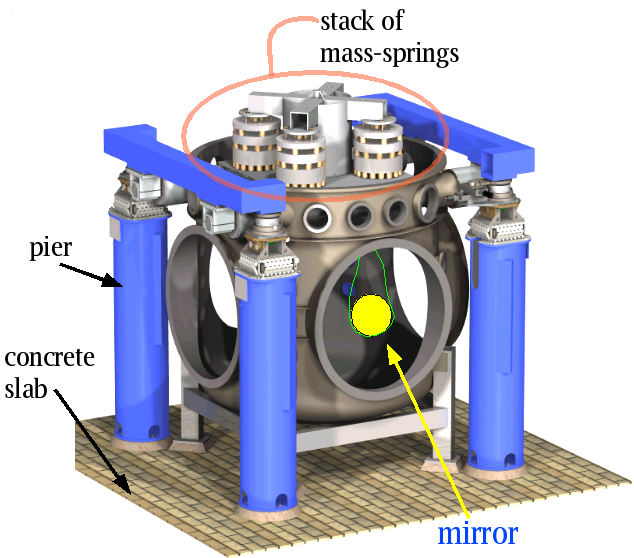
\includegraphics[angle=0,width=6.5in]{Figures/AppG/BSC.png}}
\caption[BSC Stack]{A Schematic Diagram of an isolation stack.}
\label{fig:BSC}
\end{figure}



\section{Pre-Stabilized Laser}
\label{sec:PSL}

Before the laser beam enters the interferometer it is conditioned in several ways
by both in-vacuum and out of vacuum optics.

The Pre-Stabilized Laser (PSL) sub-system consists of: the 10 W CW Nd:YAG laser,
a fixed reference cavity for frequency stabilization, a triangular,
'pre-mode cleaner' cavity which passively filters laser noise above 1 MHz, and
an intensity stabilization servo which actively quiets laser power fluctuations below
100 kHz.

\subsection{Laser}

The interferometer is illuminated by a Master-Oscillator, Power Amplifier (MOPA) 
style Nd:YAG laser which has a nominal output power of 10 W~\cite{Rick:Laser}. The
laser was purchased from Lightwave Electronics~\footnote{
\href{http://www.lwecorp.com}{http://www.lwecorp.com}}. It uses a Model
126-1064-700 NPRO (Non-Planar Ring Oscillator) as the master oscillator and a 
double pass through a set of Nd:YAG rods for the amplifier.

\subsection{Frequency Stabilization Servo (FSS)}

The purpose of the Frequency Stabilization Servo (FSS) is to suppress the
frequency (phase) fluctuations of the laser from 0-100 kHz and to provide
a wide bandwidth frequency actuator for inputs from the main interferometer.
The place of the FSS within the interferometer's overall frequency stabilization
scheme is shown in {Figure~\ref{fig:CMblock}.}

\subsubsection{AOM}

A small fraction ($\sim$10 mW) of the laser light is picked off and locked to a
fixed reference cavity after double passing through an Acousto-Optic
Modulator (AOM) as shown in Figure~\ref{fig:CMblock}. The AOM is just
a crystal with a PZT bonded to it. The PZT is driven at 80 MHz by a high
power RF source to set up a standing acoustic wave in the crystal. The varying
density fluctuations in the crystal act like a transmissive diffraction grating.
The resulting first order diffracted beams have a frequency shift relative to the incident
carrier which is equal to the RF drive frequency. The spherical mirror catches
only the first-order beam (the +1 beam in the diagram) and redirects it to the
crystal where it gets diffracted again, but this time along back along the path
of the incident carrier. The light which finally gets to the reference cavity
has experienced a frequency shift equal to twice the AOM drive frequency.

\subsubsection{Reference Cavity}

The reference cavity is a 200 mm long, monolithic, fused silica cylinder, 
with mirrors of equal reflectivity optically contacted onto each end. 
The entire cylinder is suspended
by springs from a set of posts mounted to a stack of stainless steel plates.
The three plates are separated by RTV (Room Temperature Vulcanizing) silicone
spacers which act as springs to provide further seismic
isolation. The pendulum mode resonance of the cavity/spring system is 
damped by eddy current damping between the cavity and the first stack layer.
This entire assembly is mounted in a small ($\sim$1 m) vacuum chamber which is
pumped down to an ultra-high vacuum by an ion pump.

The cavity must be isolated from the environment well enough to serve as a quiet
wavelength reference. The total frequency noise coming out of the FSS is 
dominated by sources other than the cavity displacement noise: acoustic band 
vibrations of the steering optics on the
optical table (80 mHz/$\sqrt{\mbox{Hz}}$ at 50-1000 Hz) and electronics noise in the 
VCO driving the AOM (20 mHz/$\sqrt{\mbox{Hz}}$, broadband). From these measurements of the
output noise of the FSS system, we can place an upper limit on the reference
cavity displacement noise 

\begin{equation}
\delta x  <  \left(\frac{20 \, \mbox{mHz}/\sqrt{\mbox{Hz}}}
                   {3 \times 10^{14} \, \mbox{Hz}} \right)
                   \times \left(L_{RefCav} \approx 20 cm \right)
\end{equation}
which is $\sim5 \times 10^{-17} \mbox{m}/\sqrt{\mbox{Hz}}$.

As shown in Appendix~\ref{app:ModeCleaner}, the frequency noise coming
out of the FSS is not a significant component of what actually gets
to the inteferometer since the the Mode Cleaner is able to suppress the
FSS noise enough below a few kHz. Further work needs to be done in the
$\sim$3-7 kHz band on either the VCO noise or the MC servo gain in order
to meet the requirement for the frequency noise incident on the interferometer.


\subsection{Pre-Mode Cleaner (PMC)}

The PMC is a triangular ring cavity made by optically contacting
three mirrors to a rigid, fused silica spacer. The main purpose of this
cavity is to passively filter amplitude and phase fluctuations of the
laser at the resonant sideband frequency ($\sim$25 MHz) which is used
for the gravitational wave readout. The in-vacuum Mode Cleaner must transmit 
these sidebands and so it provides no filtering of noise at this frequency.
Since there are no active stabilization servos with enough bandwidth 
to act at 25 MHz, the PMC must do all of the filtering.

The PMC has a cavity pole at $\sim$1 MHz, reducing the 
laser noise by a factor of 25 at the sideband frequency.

\subsection{Intensity Stabilization Servo (ISS)}

The ISS senses a fraction of the laser power and feeds back the AC component
of this signal to the laser, in order to suppress power fluctuations from
1-100,000 Hz. The feedback actuator is a current shunt~\cite{PK:CS} which
modulates the current going into the laser diodes which pump the MOPA's
power amplifier. This actuator has a $\sim2$ kHz bandwidth.

Based upon the requirements for the laser intensity noise described
in Section~\ref{sec:IntensityNoise} and the intensity noise trace in
Figure~\ref{fig:S3noise}, we know that the existing servo is not 
sufficient to allow interferometer operation at the designed noise level.

A new servo with more gain and dynamic range is currently being designed.
It is expected that the new servo will suppress the laser intensity noise
contribution to below 1/10 of the Science Requirement.


\section{Input Optics}
\label{app:IOO}

The Input Optics sub-system consists of three major components:

\begin{itemize}
\item   Modulators. The phase modulation sidebands used to sense the
        interferometer lengths and angles are applied by passing the
        beam through commercial (New Focus Model 4003) Pockels cells
        made of MgO:LiNbO$_3$ crystals. 
        A tunable inductor is attached to the crystal to form a resonant
        LC circuit with the crystal capacitance at the modulation
        frequency.
\item   A Mode Cleaner (detailed in Appendix~\ref{app:ModeCleaner})
\item   Faraday Isolator. An in-vacuum Faraday rotator is mounted rigidly to
        to the top of a HAM isolation stack between the suspended Mode Cleaner
        and the suspended Mode Matching Telescope.
\item   Mode Matching Telescope. This suspended, three mirror telescope expands
        the beam exiting the Mode Cleaner and matches it to the resonant mode
        of the interferometer arms.
\end{itemize}



%\section{Vacuum}

%The commissioning of the vacuum system was thankfully not a part of this thesis;
%this description is included only for completeness.

%The vacuum system consists of large chambers to house the optics, vacuum pumps to 
%attain and maintain the ultra-high vacuum state, and most notably, 4 km beam 
%tubes to house the interferometer arms.


%\begin{itemize}
%\item     Tubes (what kind of steel, diameter, thickness)
%\item     b. Chambers with viewports
%\item     c. Pumps (rough, turbo, cryo)
%\item     Gate Valves
%\end{itemize}

%There are two chamber designs used in LIGO. The Basic Symmetric Chamber (BSC)
%houses the main interferometer optics and has one more stage of seismic
%isolation than the Horizontal Access Module (HAM) which houses the mode
%matching telescope, the mode cleaner, the recycling mirror, and the AS
%port output telescope.

%The vacuum for the arms is contained by 1.2 m diameter tubes made of 3 mm
%thick 304L stainless steel \cite{Rai:Tubes,Rai:Leaks}.
